% Eine dokumentierte Version der Video Datei zum achzehnten
% Teil des LaTeX Tutorials.

\documentclass[12pt,a4paper,bibtotoc]{scrreprt}

% Alle meine üblichen Paketdefinitionen lade ich
% mit 'input' hinzu:
% Paketdefinitionen für deutsche LaTeX Dokumente

% Pakete um deutsche Texte in LaTeX zu setzen:

% Wir setzen einen Text in neuer deutscher
% Rechtschreibung:
\usepackage[ngerman]{babel} 
% Eingabetext ist im utf-8 Format:
\usepackage[utf8]{inputenc} 
% Korrektes Ausgabeencoding für deutsche
% Umlaute:
\usepackage[T1]{fontenc} 
% Korrekte Anführungsstriche in deutschen Texten: 
\usepackage{csquotes} 

% Pakete für den Mathematikmodus:
\usepackage{amsmath}
\usepackage{amssymb}
% Zum Setzen von Einheiten
\usepackage{siunitx} 
% Wir wollen Zahlen/Einheiten nach
% deutschen Regeln setzen. siunitx nimmt
% leider nicht direkt die babel Spracheinstellung
\sisetup{locale = DE} 

% Figuren speichern wir immer in einem Unterordner
% 'figuren' unter unseren LaTeX Dokumenten
\usepackage{graphicx}
\graphicspath{{figuren/}}

% Das Paket biblatex ist für Literaturverweise
% zuständig.
\usepackage[backend=biber,   
            style=alphabetic % alphabetischer Zitierstil
           ]{biblatex}
           
% Meine Literaturdatenbank:
\addbibresource{literatur.bib}

% Sonstiges:

% Das Paket xspace sorgt für 'intelligente'
% Leerzeichnsetzung nach einem LaTeX Makro.
% siehe auch Datei my_newcommands_german.tex
\usepackage{xspace}

% Hin und wieder benötige ich ein wenig Dummy
% Text zum Vorführen wie hier in den Videos:
\usepackage{blindtext}

% Das Paket fancyhdr (fancyheaders) erlaubt eine
% umfangreiche Konfiguration von Dokument Kopf-
% und Fusszeilen:
\usepackage{fancyhdr}
\pagestyle{fancy}
\fancyfoot{}
\fancyfoot[LE,RO]{\thepage}

% Beachten Sie dass für ein gedrucktes Dokument
% PDF-Links wenig Sinn machen! Daher erscheinen
% in dieser Version keine hyperref Befehle!


% Meine Definitionen neuer LaTeX Kommandos:
% Einige nützliche newcommand Definitionen
% für deutsche LaTeX Texte

% Abkürzungen für 'zum Beispiel', 'unter anderem'
% etc. In diesen Abkürzungen ist das Leerzeichen
% zwischen den Buchstaben kleiner als
% normalerweise. Deswegen wird dieses
% mit '\,' anstatt mit einem space gesetzt.
% Abgeschlossen werden die Definitionen durch ein
% \xspace so dass, wenn nötig,
% im Text ein Leerzeichen nach den Makros eingefügt
% wird.
\newcommand{\zB}{z.\,B.\xspace} % zum Beispiel (z. B.)
\newcommand{\ua}{u.\,a.\xspace} % unter anderem (u. a.)
\newcommand{\uU}{u.\,U.\xspace} % unter Umständen (u. U.)

% Kurzformen für existierende, lange LaTeX Befehle:
\newcommand{\tb}{\textbackslash}

% Kommandos für Verweise (ref) Befehle:
\newcommand{\chapterref}[1]{Kapitel~\ref{#1}}
\newcommand{\sectionref}[1]{Abschnitt~\ref{#1}}
\newcommand{\subsectionref}[1]{Unterabschnitt~\ref{#1}}
\newcommand{\equationref}[1]{Gl.~(\ref{#1})}
\newcommand{\figureref}[1]{Figur~\ref{#1}}
\newcommand{\tableref}[1]{Tabelle~\ref{#1}}

% Kommandos für Mathemtikkonstrukte:

% Betragsstriche mit korrekter Größe um jedes Objekt:
\newcommand{\abs}[1]{\left|#1\right|}

% Ableitungen mit aufrecht gedruckten Differentialoperator:
\newcommand{\deriv}[2]{\frac{\mathrm{d} #1}{\mathrm{d} #2}}

% Aufrecht gedruckte Eulersche Zahl und imaginäre Einheit:
\newcommand{\euler}{\mathrm{e}}
\newcommand{\imag}{\mathrm{i}}


% Titel und Autor:
\title{Ein größeres Dokument}
\author{Thomas Erben}
\date{\today}

% Sie können nur bestimmte Kapitel mit 'includeonly'
% kompilieren:
%\includeonly{Kapitel_Hobbit}

% Man kann auch mehrere Kapitel via 'includeonly'
% einbinden:
%\includeonly{Kapitel_Hobbit,Kapitel_Mathematik}

\begin{document}
%
\maketitle
%
\tableofcontents
%
% Man beachte dass in der Ausgabe vor jedem
% 'include' eine neue Seite angefangen wird.
% Wenn man sein Dokument nach Kapiteln aufspaltet
% faellt dies nicht auf da auch Kapitel auf neue
% Seiten gesetzt werden.
%
\chapter{Bevor es losgeht}
%
\section{Vorwort}
Hier versuchen wir ein längeres Dokument mit dem Material vorheriger
Tutorials zusammenzusetzen. Onlinematerialien zu den Tutorials finden Sie
unter \url{https://github.com/terben}.
%
\section{Einleitung}
Im folgenden haben wir eine bunte Zusammenstellung an Text mit
wichtigen \LaTeX{}-Elementen. In \sectionref{sec:literatur} zeigen wir
Literaturverweise, in \chapterref{chap:hobbit} sprechen wir über den
kleinen Hobbit. Dabei zeigen wir in
\sectionref{sec:zwerge} die \tableref{tab:zwerge}. \chapterref{chap:mathematik}
bespricht einige mathematische Formeln. In \figureref{fig:trigo_funk}
und \figureref{fig:kreis_quadrat} sehen wir zwei eingebundene Figuren.
%
\section{Dummy Text}
\blindtext
\blindtext
%

%
\chapter{\LaTeX{}-Textelemente}
\label{chap:latex_elemente}
%
\section{Texthervorhebungen}
Windows und Linux sind gute Betriebssysteme.  \\
Windows und Linux sind \emph{gute} Betriebssysteme.  \\
Windows und Linux sind \textbf{gute} Betriebssysteme.  \\
\texttt{Windows} und \texttt{Linux} sind
\emph{\textbf{gute}} Betriebssysteme.  \\
%
\section{Anführungsstriche}
Thomas sagte "Guten Morgen" (falsch!). \\
Thomas sagte \enquote{Guten Morgen} (richtig!).
%
\section{Aufzählungen}
%
Hier eine \LaTeX{} Aufzählung:
\begin{enumerate}
  \item Vor dem ersten Punkt
  \item Erster Punkt
  %
  \begin{enumerate}
    \item Erster Unterpunkt
    \item Zweiter Unterpunkt
  \end{enumerate}
  \item Zweiter Punkt
  \item Dritter Punkt   
\end{enumerate}
%
\section{Literaturzitate}
\label{sec:literatur}
Studienanfänger der Physik benutzen oft \cite{gerthsen2013physik} als
Einführungstext in die Experimentalphysik. Für \LaTeX{} verwenden wir
den Onlinetext \cite{daniel2015l2kurz}. Während oder nach der
Masterarbeit schreiben wir vielleicht auch mal eine Veröffentlichung
wie hier in \cite{heymans2006shear}.
%
\section{Ein paar Elemente mehr}
\blindtext[2]
\blindlist{itemize}
\blindtext[2]
\blindlistlist[3]{itemize}

%
\chapter{Der kleine Hobbit}
%
\label{chap:hobbit}
Nachdem wir in \chapterref{chap:latex_elemente} einige \LaTeX{}-Elemente
früherer Videos zusammengefasst haben schreiben wir hier etwas über den
kleinen Hobbit. In \chapterref{chap:mathematik} geht es anschließend
mit Mathematik weiter.

Hier noch etwas mehr Text. Hier tippe ich jetzt weiter.
%
\section{Eine unvorhergesehene Gesellschaft}

\subsection*{Die Hobbithöhle}
In einer Höhle in der Erde, da lebte ein \textbf{Hobbit}. Nicht in
einem schmutzigen, nassen Loch, in das die Enden von irgendwelchen
Würmern herabbaumelten und das nach Schlamm und Moder roch. Auch nicht
etwa in einer trockenen Kieshöhle, die so kahl war, dass man sich
nicht einmal niedersetzen oder gemütlich frühstücken konnte. Es war
eine \underline{Hobbithöhle}, und das bedeutet Behaglichkeit.

Diese Höhle hatte eine kreisrunde Tür wie ein Bullauge. Sie war grün
gestrichen, und in der Mitte saß ein glänzend gelber Messingknopf. Die
Tür führte zu einer röhrenförmig langen Halle, zu einer Art Tunnel,
einem Tunnel mit getäfelten Wänden.

\subsection*{Ein guter Morgen (?)}
Alles, was also der keineswegs misstrauische Bilbo an diesem Morgen
sah, war ein kleiner, alter Mann mit einem Stab, hohem, spitzem blauen
Hut, einem langen, grauen Mantel, mit einer silbernen Schärpe, über
die sein langer, silberner Bart hing, ein kleiner, alter Mann mit
riesigen schwarzen Schuhen.

\enquote{Guten Morgen}, sagte Bilbo, und er meinte es ehrlich. Die
Sonne schien, und das Gras war grün. Aber Gandalf schaute ihn scharf
unter seinen buschigen Augenbrauen hervor an.

\enquote{Was meint Ihr damit?} fragte er. 
\begin{itemize}
  \item \enquote{\emph{Wünscht Ihr mir einen guten Morgen?}}

  \item \enquote{\emph{Oder meint Ihr, dass dies ein guter Morgen
        ist, gleichviel, ob ich es wünsche oder nicht?}}
  \item \enquote{\emph{Meint Ihr, dass Euch der Morgen gut bekommt?}}
  \item \enquote{\emph{Oder dass dies ein Morgen ist, an dem man gut
        sein muss?}}
\end{itemize}

\enquote{Alles auf einmal}, sagte Bilbo. \enquote{Wie heißt Ihr
  eigentlich?} fragte der Hobbit. \enquote{Ich bin Gandalf, und Gandalf,
denkt nur, das bin ich!} antwortete der Zauberer.
%
\section{Die Zwerge}
\label{sec:zwerge}
Mit dem Namen Gandalf fiel bei Bilbo der Groschen. Der Zauberer war
früher oft zu Gast bei den Hobbits. Er hatte seinem Grossvater vor
Ewigkeiten ein paar magische Diamantenklammern geschenkt und die
Hobbits zur Sommersonnenwende stets mit beeindruckenden Feuerwerken
erfreut. Nach einer Weile lud Bilbo den Zauberer für den nächsten Tag
zum Tee ein und dieser verschwand so schnell wie er gekommen war.
 
Bevor Gandalf am folgenden Nachmittag erschien, wurde der arme Hobbit
von 13 ungebetenen Gästen, es waren Zwerge, heimgesucht. Ihre Namen
finden sich, zusammen mit einigen Zusatzinformationen, in
Tabelle~\ref{tab:zwerge}.
% 
\begin{table}
  \centering
  % Die folgenden zwei Befehle erzeugen eine Tabellenüberschrift
  \captionabove{Die dreizehn Zwerge}
  \label{tab:zwerge}
  \begin{tabular}{l||l|l|l|l|l}
  Name   & Bart & Gürtel & Kapuze & Instrument & Sonstiges \\
  \hline
  Dwalin & blau & gold & dunkelgrün & Bratsche & \\
  Balin & weiß & & purpurrot & Bratsche & \\
  Kili & gelb & silber & blau & Fiedel & Werkzeug \\
  Fili & gelb & silber & blau & Fiedel & Spaten \\
  Dori & & gold & purpurrot & Flöte & \\
  Nori & & gold & purpurrot & Flöte & \\
  Ori & & gold & grau & Flöte & \\
  Oin & & silber & braun & & \\
  Gloin & & silber & silber & & \\
  Bifur & & & gelb & Klarinette & \\
  Bofur & & & gelb & Klarinette & \\
  Bombur & & & blaßgrün & Trommel & fett \\
  Thorin & & & himmelblau mit & Harfe & sehr berühmt \\
         & & & silberner Schärpe & &
  \end{tabular}
\end{table}
%

%
\chapter{Mathematik}
\label{chap:mathematik}
%
\section{Mathematischer Formelsatz}
Seien \begin{math}x\in\mathbb{R}\end{math} und
$y\in\mathbb{R}$ dann gilt
%
\begin{equation}
  |x+y| \leq |x| + |y|.
\end{equation}
%
Auch mehrzeilige Gleichungen sind möglich:
%
\begin{align}
  (a+b)^{2} & = (a+b)(a+b) \\
           & = a^{2}+2ab+b^{2}
\end{align}
Es gibt auch abgesetzte Formeln ohne Nummern:
%
\begin{equation*}
  \int_{0}^{\pi/4}\sin(x)\,\mathrm{d}x=
  1-\frac{1}{\sqrt{2}}
\end{equation*}
Für abgesetzte Formeln ohne Nummern gibt es auch eine Kurzform:
%
% So, hier noch die etwas kompliziertere Formel:
\[
  R=\frac{\sum_{i=1}^{n}(x_{i}-\bar{x})(y_{i}-\bar{y})}{\left[\sum_{i=1}^{n}(x_{i}-\bar{x})^{2}\sum_{i=1}^{n}(y_{i}-\bar{y})^{2}\right]^{1/2}}
\]
%
\section{Trigonometrische Funktionen}
\label{sec:trigo_funk}
Die folgenden Sätze über Sinus und Cosinus stammen hauptsächlich
von Wikipedia.

Sinus- und Cosinusfunktion sind elementare mathematische Funktionen.
Vor Tangens und Cotangens bilden sie die wichtigsten trigonometrischen
Funktionen. Sinus und Cosinus werden unter anderem in der Geometrie
für Dreiecksberechnungen in der ebenen und sphärischen Trigonometrie
benötigt. Auch in der Analysis sind sie wichtig. Wellen wie
Schallwellen, Wasserwellen und elektromagnetische Wellen lassen sich
als aus Sinus- und Cosinuswellen zusammengesetzt beschreiben, sodass
die Funktionen auch in der Physik als harmonische Schwingungen
allgegenwärtig sind. Tangens und Cotangens sind als Quotienten von
Sinus und Cosinus definiert und spielen eine ähnlich wichtige Rolle
wie Sinus und Cosinus. Alle vier Funktionen sind in
Abbildung~\ref{fig:trigo_funk} im Bereich $x\in[0, 2\pi]$ dargestellt.
%
\begin{figure}[ht]
  \centering
  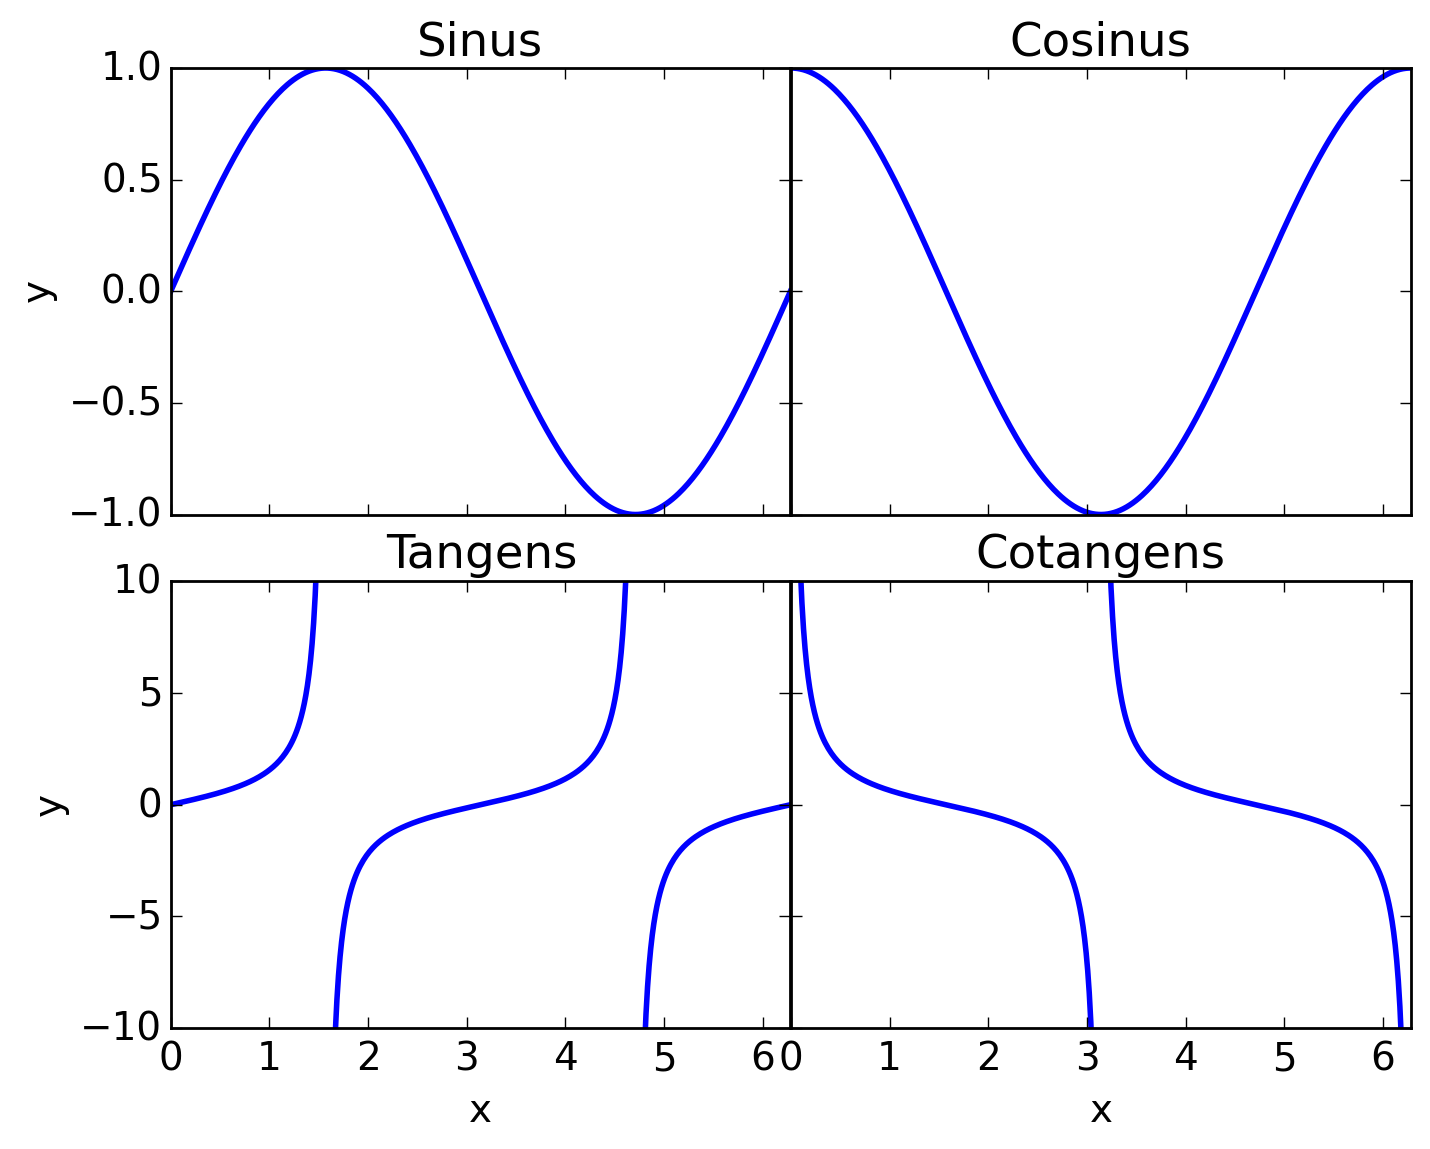
\includegraphics[width=0.9\textwidth]{trigo_funktionen}
  \caption{Trigonometrische Funktionen: Gezeigt sind die Sinusfunktion
    (oben links), die Cosinusfunktion (oben rechts), der Tangens
    (unten links) und der Cotangens (unten rechts).}
  \label{fig:trigo_funk}
\end{figure}
%
\section{Kreis und Quadrat}
Ein Kreis ist eine ebene geometrische Figur. Er wird definiert als die
Menge aller Punkte einer Ebene, die einen konstanten Abstand zu einem
vorgegebenen Punkt dieser Ebene (dem Mittelpunkt) haben. Der Abstand
der Kreispunkte zum Mittelpunkt ist der Radius oder Halbmesser des
Kreises, er ist eine positive reelle Zahl. Der Kreis gehört zu den
klassischen und grundlegenden Objekten der euklidischen Geometrie.

In der Geometrie ist ein Quadrat (veraltet auch Geviert) ein
spezielles Polygon, nämlich ein ebenes, konvexes und regelmäßiges
Viereck.

Kreis und Quadrat sind in \figureref{fig:kreis_quadrat}
\emph{korrekt} dargestellt.
%
\begin{figure}[ht]
  \centering
  % Wir fassen zwei Figuren zu einer zusammen. Damit so nebeneinander
  % gesetzt werden darf die Gesamtbreite der Figuren '\textwidth'
  % nicht überschreiten.
  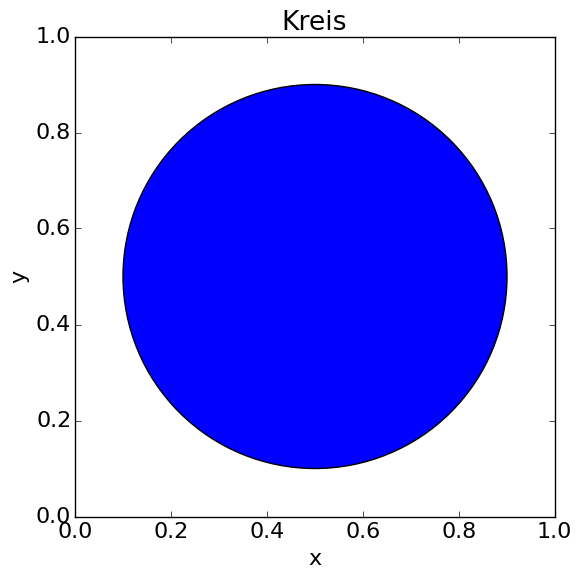
\includegraphics[width=0.45\textwidth]{kreis}
  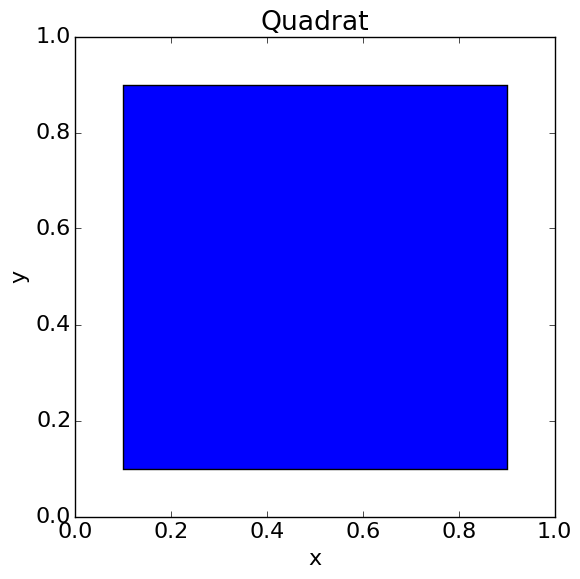
\includegraphics[width=0.45\textwidth]{quadrat}
  \caption{Kreis (links) und Quadrat(rechts) mit korrekter Skalierung}
  \label{fig:kreis_quadrat}
\end{figure}
%

%
\printbibliography
\end{document}
